\documentclass{article}

\usepackage[utf8]{inputenc}
\usepackage[T1]{fontenc}

\usepackage{geometry}
 \geometry{
 a4paper,
 total={170mm,257mm},
 left=20mm,
 top=20mm,
 }

\setlength{\parskip}{7pt}
\setlength{\parindent}{0pt}

\title{RISC-V external debugging}
\date{2019-10-18}

\PassOptionsToPackage{hyphens}{url}\usepackage{hyperref}
\usepackage{listings}
\usepackage{amssymb}
\usepackage{graphicx}
\graphicspath{ {./images/} }
\usepackage{float}

\lstset{
	basicstyle=\ttfamily,
	breaklines=true,
	columns=fullflexible,
	tabsize=4,
	showstringspaces=false,
	frame=single
}

\begin{document}
	\maketitle
	
	\section{About}
	
	This document gives an overview of an external debug system for RISC-V targets. Debug interfaces can be found in several RISC-V platforms, as can be seen in the following examples:
	
	\begin{figure}[H]
   	\centering
   	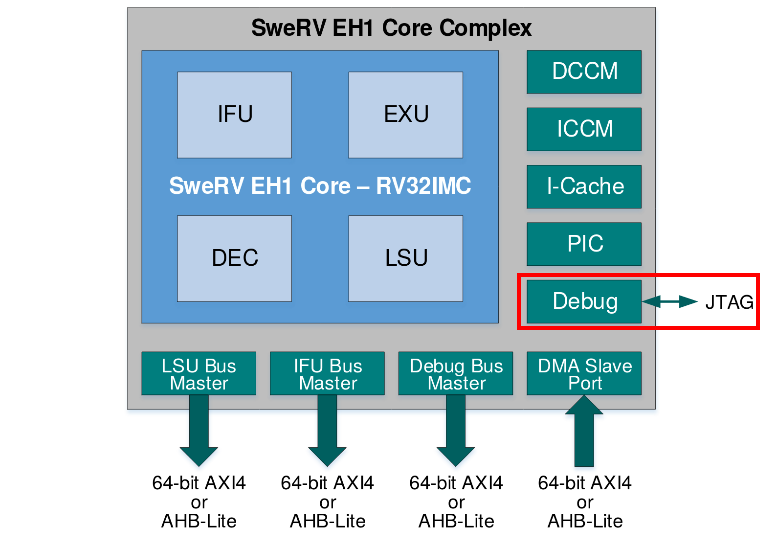
\includegraphics[width=0.65\textwidth]{swerv.png}
   	
   	SweRV EH1 Core Overview - \url{https://github.com/westerndigitalcorporation/swerv_eh1}
	\end{figure}
	
	\begin{figure}[H]
   	\centering
   	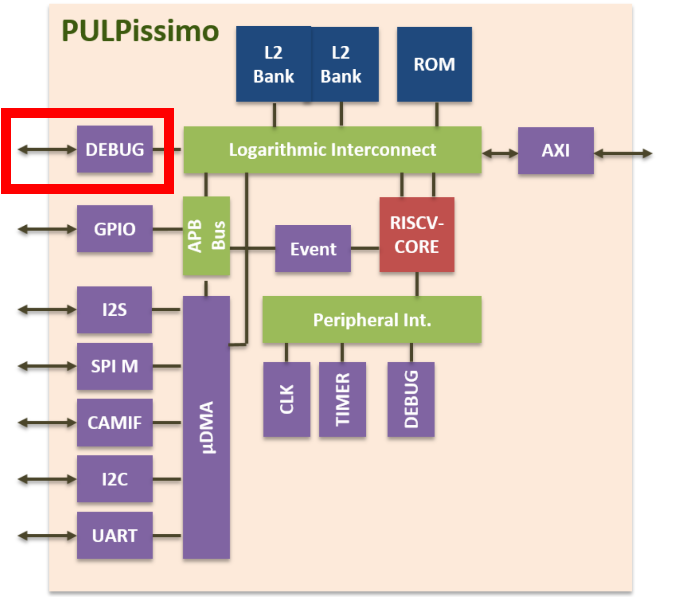
\includegraphics[width=0.55\textwidth]{pulpissimo.png}
   	
   	Pulpissimo platform architecture - \url{https://github.com/pulp-platform/pulpissimo}
	\end{figure}
	
	\newpage
	\section{Overview}
	
	The external part of the debug system is the following:
	
	\begin{figure}[H]
   	\centering
   	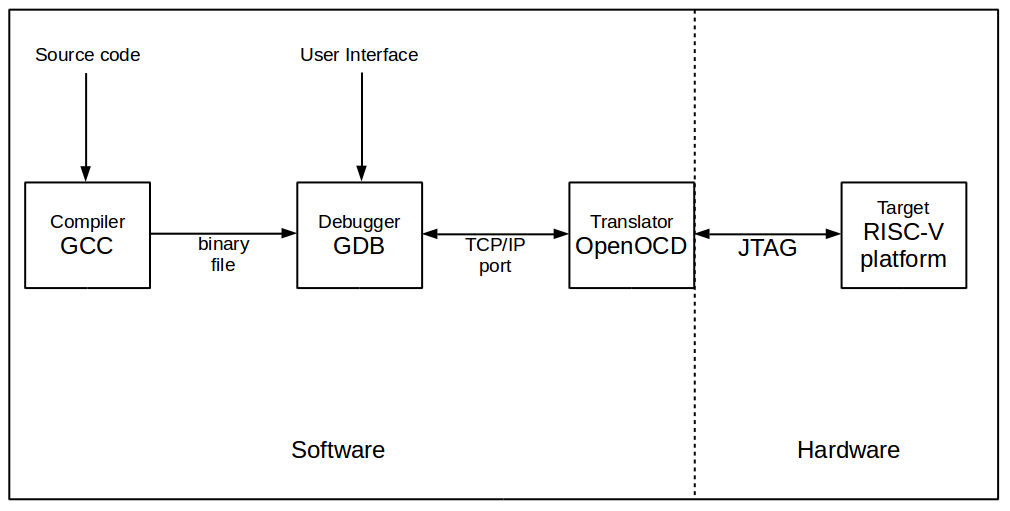
\includegraphics[width=.8\textwidth]{debug-system-overview.png}
	\end{figure}
	
	\begin{figure}[H]
   	\centering
   	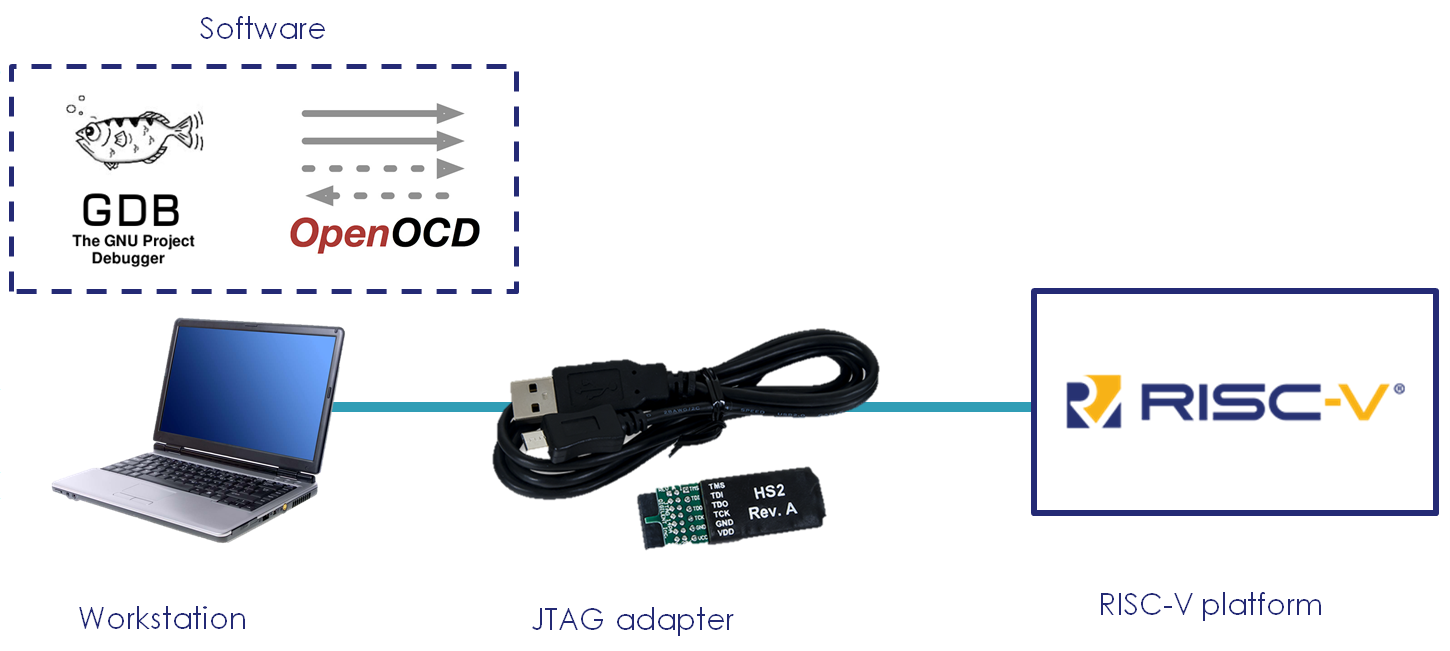
\includegraphics[width=.8\textwidth]{debug-pictures.png}
	\end{figure}
	
	\vspace{-\topsep}
	\begin{itemize}
	\item \textbf{Compiler}: binary production from source code
	\item \textbf{Debugger}: user interface and debug capabilities
	\item \textbf{Translator}: translation of debug commands into hardware commands
	\item \textbf{Transport}: hardware link
	\item \textbf{Target}: the RISC-V platform
	\end{itemize}
	
	Several choices are available for each of these components. A possible choice with free software is:
	
	\vspace{-\topsep}
	\begin{itemize}
	\item The \textbf{GNU toolchain} provides GCC and GDB and has been ported for RISC-V
	\item \textbf{OpenOCD} stands for Open On Chip Debugging and provides debugging and in-system programming. RISC-V support has been added.
	\item \textbf{JTAG} is currently the most popular debug interface on RISC-V platforms.
	\end{itemize}
	
	Links:
	
	\url{https://github.com/riscv/riscv-gnu-toolchain}
	
	\url{https://github.com/riscv/riscv-openocd}
	
	
	\newpage
	\section{Example}
	
	This is a generic example of using the debug system. Details and adaptaions would need to be added to work with a specific implementation. It is essentially the example given by Spike (\url{https://github.com/riscv/riscv-isa-sim#debugging-with-gdb}).
	
	The test program is called rot13.c :
	
	\begin{lstlisting}[language=C]
	char text[] = "Vafgehpgvba frgf jnag gb or serr!";
	
	// Don't use the stack, because sp isn't set up.
	volatile int wait = 1;
	
	int main()
	{
	    while (wait)
	        ;
	
	    // Doesn't actually go on the stack, because there are lots of GPRs.
	    int i = 0;
	    while (text[i]) {
	        char lower = text[i] | 32;
	        if (lower >= 'a' && lower <= 'm')
	            text[i] += 13;
	        else if (lower > 'm' && lower <= 'z')
	            text[i] -= 13;
	        i++;
	    }
	
	done:
	    while (!wait)
	        ;
	}
    \end{lstlisting}
    
    We use GCC to compile it.
    
    \begin{lstlisting}[language=bash]
	$ riscv32-unknown-elf-gcc -g -Og <other options> -o rot13-32 rot13.c
    \end{lstlisting}
    
    The RISC-V platform is started and made ready to enter debug mode.
    
    A JTAG debug adapter is connected between the workstation and the target.
    
    We launch OpenOCD with a configuration file appropriate for the debug adapter:
    
    \begin{lstlisting}[language=bash]
	$ openocd -f <config file>
	Open On-Chip Debugger 0.10.0+dev-00630-g30b93b8-dirty (2019-09-02-16:40)
	Licensed under GNU GPL v2
	[...]
	Info : Listening on port 3333 for gdb connections
	Info : Listening on port 6666 for tcl connections
	Info : Listening on port 4444 for telnet connections
    \end{lstlisting}
    
    \newpage
    In a separate shell, the GDB session is started:
    
    \begin{lstlisting}[language=bash]
	$ riscv32-unknown-elf-gdb rot13-32
	GNU gdb (GDB) 8.0.50.20170724-git
	Copyright (C) 2017 Free Software Foundation, Inc.
	License GPLv3+: GNU GPL version 3 or later <http://gnu.org/licenses/gpl.html>
	This is free software: you are free to change and redistribute it.
	There is NO WARRANTY, to the extent permitted by law.  Type "show copying"
	and "show warranty" for details.
	This GDB was configured as "--host=x86_64-pc-linux-gnu --target=riscv32-unknown-elf".
	Type "show configuration" for configuration details.
	For bug reporting instructions, please see:
	<http://www.gnu.org/software/gdb/bugs/>.
	Find the GDB manual and other documentation resources online at:
	<http://www.gnu.org/software/gdb/documentation/>.
	For help, type "help".
	Type "apropos word" to search for commands related to "word"...
	Reading symbols from rot13-32...done.
	(gdb) 
    \end{lstlisting}
    
    We connect to OpenOCD, load the program and start debugging:
    
    \begin{lstlisting}[language=bash]
	(gdb) target remote localhost:3333
	Remote debugging using localhost:3333
	0x00010058 in ?? ()
	(gdb) load
	Loading section .text, size 0x98 lma 0x80000000
	Loading section .data, size 0x22 lma 0x80000098
	Loading section .sdata, size 0x4 lma 0x800000bc
	Start address 0x80000000, load size 190
	Transfer rate: 1 KB/sec, 63 bytes/write.
	(gdb) print wait
	$1 = 1
	(gdb) print wait=0
	$2 = 0
	(gdb) print text
	$3 = "Vafgehpgvba frgf jnag gb or serr!"
	(gdb) b done
	Breakpoint 1 at 0x80000080: file rot13.c, line 22.
	(gdb) c
	Continuing.
	
	Breakpoint 1, main () at rot13.c:23
	23	    while (!wait)
	(gdb) print wait
	$4 = 0
	(gdb) print text
	$5 = "Instruction sets want to be free!"

    \end{lstlisting}
	
\end{document}